\section{Experimental Studies}
\label{sec-expt}

In this section, we conducted two sets of experiments to evaluate (1) the performance of our visual processing module, (2) the accuracy of our inference module, and (3) the overall performance of our approach. 

\stitle{Experimental Setting}. %We report settings of experimental studies. 

\etitle{DataSet}. We used two datasets: (1) \kw{Soccer} dataset that we annotated; and (2) X dataset from~\cite{}. We extracted images with subjects of golf and tennis (report Statistics about the dataset). We split \kw{Soccer} (resp. X) data into two parts:{\em  I} (one third) and {\em II} (two thirds), and used {\em II} as training data, and {\em I} as testing data. 

\etitle{Queries}. We used two sets of questions: (1) the set of questions given in Table~\ref{table:questions} for \kw{Soccer} dataset; and (2) another set of questions listed in Table~\ref{} for X dataset. 

(We enlarge the training question scale from 7 into 28, so learning correlation between question and answer does not work at this time. For question details, please refer questionset.txt.rtf.)





\begin{table}[thb] 
\footnotesize
\begin{tabular}{|l|l|l|}
\hline
Id & Question                                           & Difficulty \\ \hline
%$Q_{nl_1}$  & Who is this image about?                         & Hard       \\ \hline
$Q_{nl_1}$  & Who is holding the soccer?                         & Easy       \\ \hline
$Q_{nl_2}$  & What is the uniform color of the referee?           & Easy       \\ \hline
$Q_{nl_3}$  & Is there any referee in the image?                 & Easy       \\ \hline
$Q_{nl_4}$  & Which team does the goalkeeper belong to?          & Medium       \\ \hline
$Q_{nl_5}$  & Who is the defending team?                         & Medium       \\ \hline
$Q_{nl_6}$  & Which part of the field are the players being now? & Hard       \\ \hline
$Q_{nl_7}$  & How many players are there in the image?           & Hard     \\ \hline

\multirow{2}{*}{$Q_{nl_8}$ }
 & Is this image about corner kick?           &  \multirow{2}{*}{\color{red}??}  \\ 
 & {\color{red}(If not, just list the correct one.)}  & \\ \hline
 
\multirow{2}{*}{$Q_{nl_9}$}  &   Is this image about penalty kick?  &  \multirow{2}{*}{\color{red}??}    \\ 
 & {\color{red}(If not, just list the correct one.)}  &  \\ \hline
 
\multirow{2}{*}{$Q_{nl_{10}}$}  &  Is this image about kick off?  &  \multirow{2}{*}{\color{red}??}    \\ 
 & {\color{red}(If not, just list the correct one.)}  &  \\ \hline
 
\end{tabular} 
\caption{A set of questions} \label{table:questions}
\end{table}




\subsection{Performance of Visual Task Selecting Policy }
To test the validity of reinforcement learning of selecting visual task modules, we test the inference time over accuracy with the state-of-art~\cite{VQA}~\cite{Lu2016Hie} whichi is shown in Figure~\ref{TimevsAcc}.

\begin{figure}[h]
\begin{center}
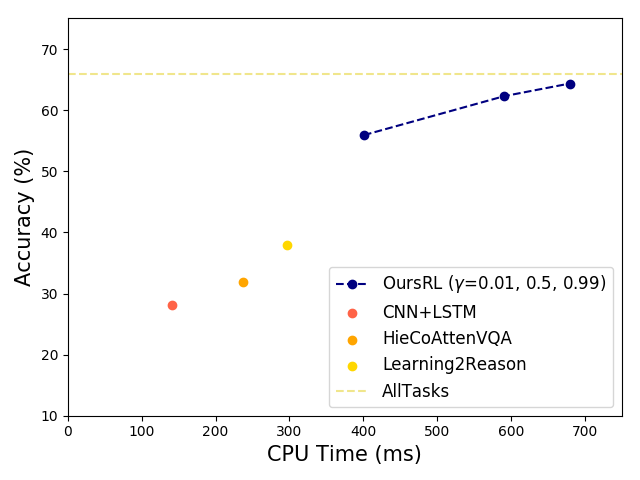
\includegraphics[width=0.9\linewidth]{TimevsAcc.png}
\end{center}
\caption{Inference Time and Accuracy}
\label{fig:TimevsAcc}
\end{figure}

Here to test the generalization, we enlarge the training set by more various question with same meaning. For instance, the original question of $Q_{nl5}$ is \textit{"Who is the defending team?"}, we add three more similar question asking \textit{Who is attacking team?}, \textit{"What is the uniform color of the defending team?"} and \textit{"What is the uniform color of the attacking team?"}. Unlike state-of-art methods answering questions in~\cite{peixi2019}, adding generalization and variation in question would not dramatically change the performance, it is because the structure is not fixed, all the visual task selection is query oriented. For~\cite{hu2017learning}, even though the network is not fixed, the answering part is based on neural network, and essentially it also learns the statically correlation, which leads to the weakness in logical reasoning.

\subsection{Effectiveness of Inference} 
\begin{figure}[tb!]
\centering
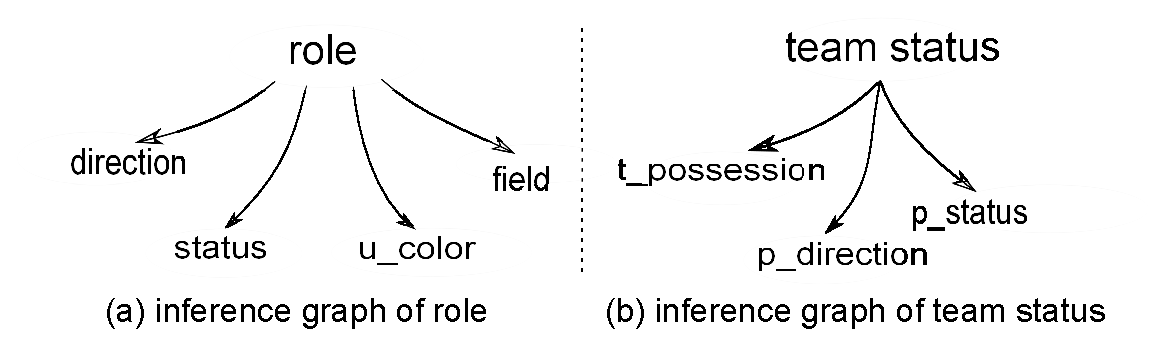
\includegraphics[width=\columnwidth]{PredictNB.eps}
\vspace{-2ex}
\caption{Inference Graphs}
\vspace{-2ex}
\label{fig:inferG}
\end{figure}
\stitle{Accuracy of Role}. Only report results with Reinforcement learning 

\stitle{Accuracy of Team-Status}. Only report results with Reinforcement learning 

\stitle{Accuracy of Kick-Off}. {\color{red} SHOW INFERENCE GRAPH AND RESULT TABLE!}

\stitle{Accuracy of Penalty Kick}. {\color{red} SHOW INFERENCE GRAPH AND RESULT TABLE!}

\stitle{Accuracy of Corner Kick}. {\color{red} SHOW INFERENCE GRAPH AND RESULT TABLE!}

\stitle{Accuracy of Attacking Free Kick}. {\color{red} SHOW INFERENCE GRAPH AND RESULT TABLE!}

\stitle{Accuracy of Balls}. {\color{red} Over new dataset. SHOW INFERENCE GRAPH AND RESULT TABLE!}

\subsection{Overall Performance}
\label{sec-overall-performance}
We use the same question setting as~\cite{peixi2019}, compared the following state-of-the-art methods: \cite{VQA},and~\cite{hu2017learning} with our method ($\gamma$=0.99), the overall performance is shown in Table~\ref{table:stateofart}. 

\begin{table}[h]
\begin{small}
\begin{tabular}{|l|l|l|l|l|}
\hline
          & CNN+LSTM & HieCoAtten & Learn2Reason & Ours  \\ \hline
$Q_{nl1}$ & 44.23    & 43.62         & 31.12        & 64.16 \\ \hline
$Q_{nl2}$ & 71.31    & 77.66         & 9.4          & 47.43 \\ \hline
$Q_{nl3}$ & 74.58    & 83.78         & 83.21        & 70.02 \\ \hline
$Q_{nl4}$ & 40.48    & 39.29         & 51.92        & 62.14 \\ \hline
$Q_{nl5}$ & 49.19    & 49.90         & 30.78        & 93.33 \\ \hline
$Q_{nl6}$ & 20.56    & 18.70         & 30.0         & 62.13 \\ \hline
$Q_{nl7}$ & 11.08    & 12.63         & 36.69        & 47.45 \\ \hline
Avg.       & 46.40    & 49.11         & 51.08        & 65.97 \\ \hline
\end{tabular}
\caption{Accuracy comparison per query (\%)}
\label{table:stateofart}
\end{small}
\end{table}

